\begin{enumerate}
    \item Perform the MiniMax algorithm on the tree in Figure 1, i.e. put a value to each node. Circle the move the root player should do.
      \begin{figure}[!ht]
      \begin{framed}
	  \centering
	  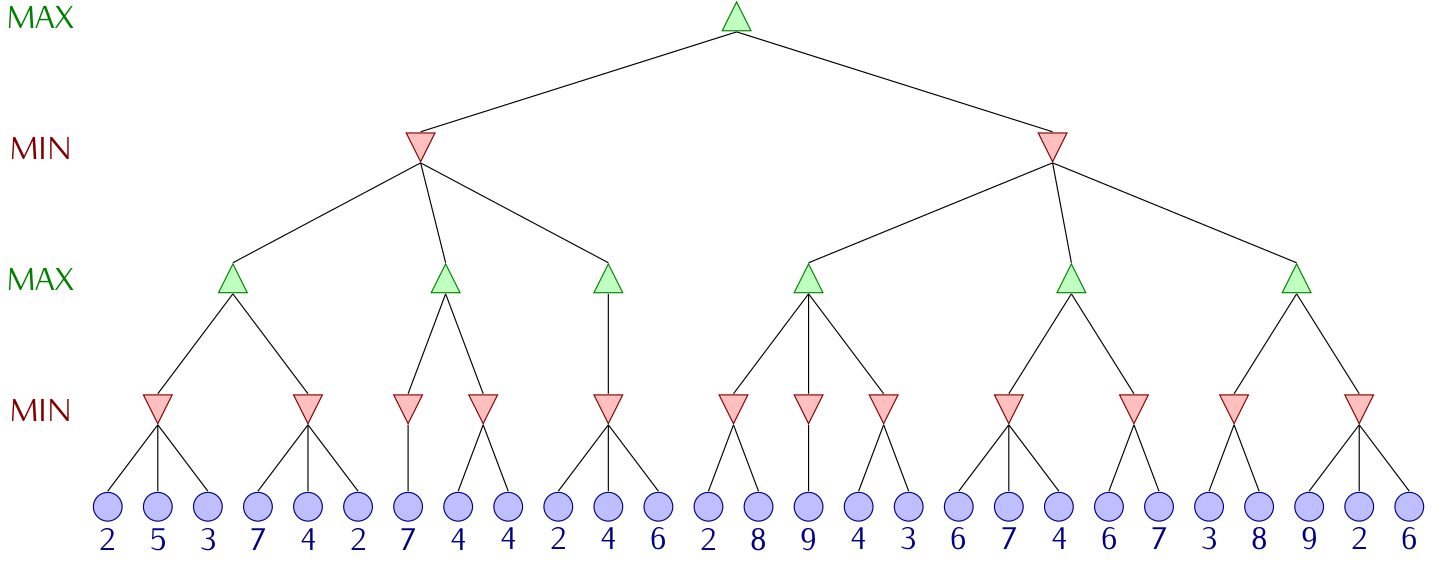
\includegraphics[width=\linewidth]{tree.png}
	  \caption{MiniMax}
      \end{framed}
      \end{figure}
      \FloatBarrier
    \item Perform the Alpha-Beta algorithm on the tree in Figure 2. At each non terminal node, put the successive values of $\alpha$ and $\beta$. Cross out the arcs reaching non visited nodes. Assume a left-to-right node expansion.
      \begin{figure}[!ht]
      \begin{framed}
	  \centering
	  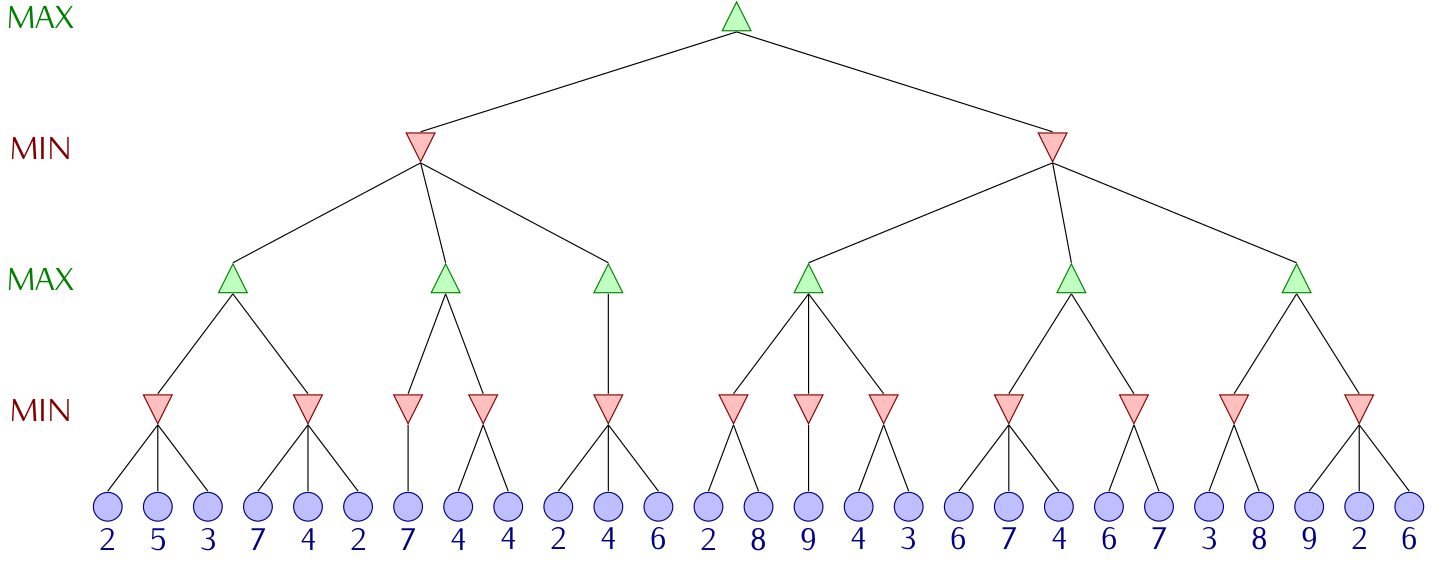
\includegraphics[width=\linewidth]{tree.png}
	  \caption{Alpha-Beta, left-to-right expansion}
      \end{framed}
      \end{figure}
      \FloatBarrier
    \item Do the same, assuming a right-to-left node expansion instead (Figure 3).
      \begin{figure}[!ht]
      \begin{framed}
	  \centering
	  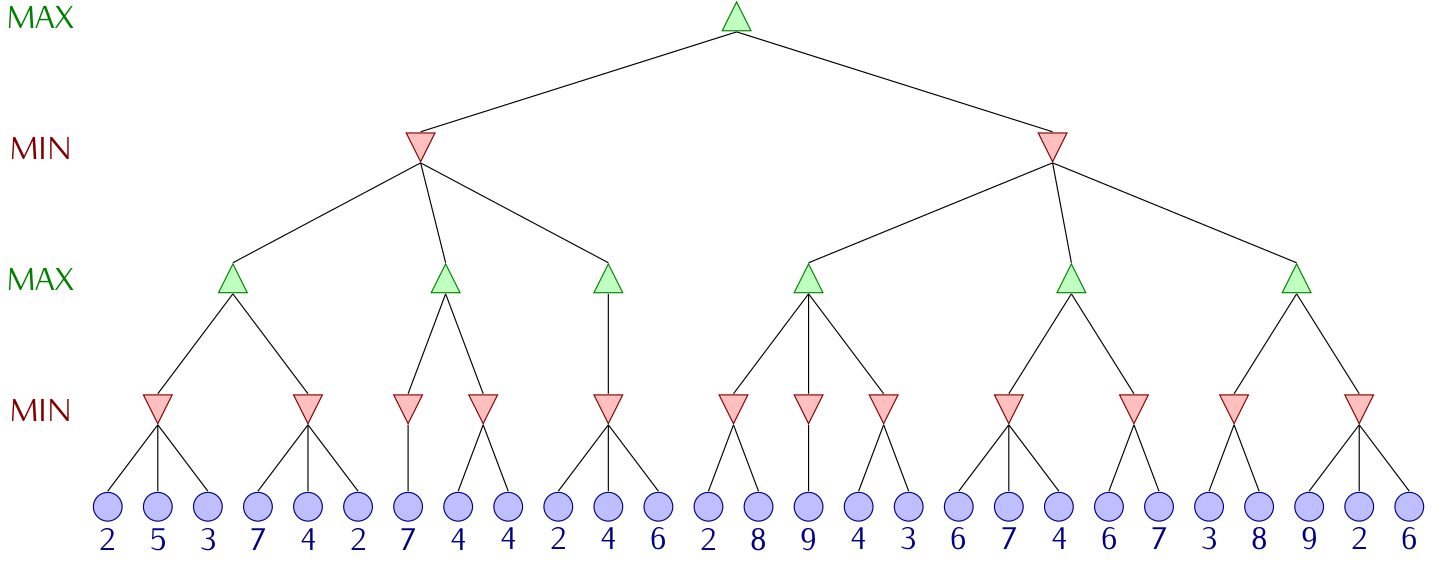
\includegraphics[width=\linewidth]{tree.png}
	  \caption{Alpha-Beta, right-to-left expansion}
      \end{framed}
      \end{figure}
      \FloatBarrier
\newpage
    \item Can the nodes be ordered in such a way that Alpha-Beta pruning can cut off more branches (in a left-to-right node expansion)? If no, explain why; if yes, give the new ordering and the resulting new pruning.
      \begin{figure}[!ht]
      \begin{framed}
        The nodes can be ordered in such a way that Alpha-Beta pruning can
        cut off more branches, as shown in the following tree:

        \bigskip
        \bigskip
	  \centering
	  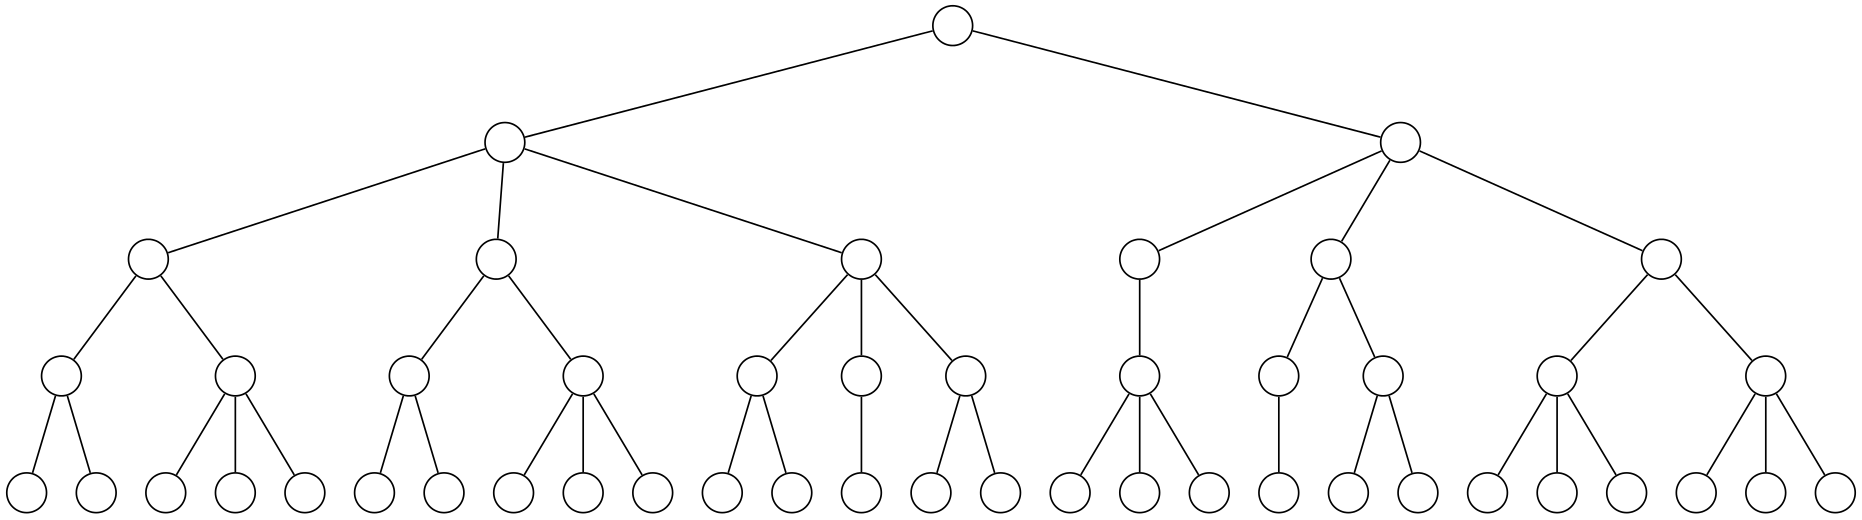
\includegraphics[width=\linewidth]{my_tree.png}
      \bigskip
      \bigskip
	  \caption{Alpha-Beta, left-to-right expansion on ordered tree}
      \end{framed}
      \end{figure}
      \FloatBarrier
    \item Launch a game where one of the agents is the basic agent described before against another agent where the basic evaluate method has been replaced such that it returns directly the result of Board.get\_score instead of -1, 0 or 1. Watch the replay of the match. What do you observe? Does one of the agent clearly overcomes the other one? Explain why there is such a difference.
      \begin{framed}
          When the new version of basic agent is Player 1, it clearly
          overcomes the old version because even with a depth of 2, the
          differences between the values evaluated are  much more relevant.
          \newline

          When the new version of basic agent is Player 2, the old basic
          agent wins because the improvement does not overcome the advantage
          from being Player 1. The first moves aren't very good but it gets
          better and better as the game enfolds catching back nearly all
          its delay at the end, losing by only 1 point. \newline
      \end{framed}
\end{enumerate}
